\documentclass{article}
% Old Thread: https://gemini.google.com/app/81401357ce6fbf66

% WRITING INSTRUCTIONS

% Please always output as follows:
% # <Section Name>
% One sentence summary of what you are about to write on the page,
% name important equations and motivation.

% One sentence about how this narrative will continue to the next
% section so that the review paper is cohesive.

% ```latex
% % Use plenty of comments in latex, so people know what you are talking about
% <the latex code>
% ```

% When writing latex, please always use:
% - \emph{} for emphasis, never boldface!
% - \begin{equation} for equations, not so much inline math
% - \begin{align} for multiline equations
% - \label and \ref for referencing equations, check narrative
% so that the text and equations are cohesive and make sense

% The sections should match the content from the presentation as well as
% the narrative and cohesion.

% Presentation Contents, for more please look at `presentation.tex`:
% 1. **Introduction**
%    - **Motivation:** Establish the need for optimization techniques in various
%      fields.
%    - **Content:** Define the optimization problem, introduce gradient descent
%      as a basic method, and discuss its limitations (ignores curvature
%      information).
%    - **Equation** Taylor first and second order to motivate methods
%    - **Equation:** Gradient descent update rule:  `x_{k+1} = x_k - α∇f(x_k)`
%      (where α is the step size).
%    - **Motivation:** Introduce Newton's method as an improvement over gradient
%      descent.
%    - **Content:** Explain how Newton's method incorporates curvature
%      information using the Hessian matrix.
%    - **Equation:** Newton's method update rule: `x_{k+1} = x_k -
%      (∇²f(x_k))⁻¹∇f(x_k)`.
%    - **Motivation:** Highlight the limitations of Newton's method
%      (computational cost, invertibility of the Hessian).

% 2. **Quasi-Newton Methods**
%    - **Motivation:** Introduce Quasi-Newton methods as a way to address the
%      limitations of Newton's method.
%    - **Content:** Explain how Quasi-Newton methods approximate the Hessian
%      matrix (or its inverse) using the BFGS algorithm.
%    - **Equation:** BFGS update rule for the approximate Hessian:
%      ```
%      B_{k+1} = B_k + \frac{y_k y_k^T}{y_k^T s_k} - \frac{B_k s_k s_k^T B_k}{s_k^T B_k s_k}
%      ```
%      where `y_k = ∇f(x_{k+1}) - ∇f(x_k)` and `s_k = x_{k+1} - x_k`.
%    - **Content:** Discuss the advantages of Quasi-Newton methods (reduced
%      computational cost, no need for Hessian inversion).

% 3. **Nonsmooth Optimization**
%    - **Motivation:** Explain the challenges of optimizing nonsmooth functions.
%    - **Content:** Define nonsmooth functions and provide examples (absolute
%      value, max function).
%    - **Content:** Discuss how gradient-based methods can struggle with
%      nonsmooth functions (oscillations, slow convergence).
%    - **Motivation:** Introduce line search as a technique to improve
%      optimization in nonsmooth cases.
%    - **Content:** Explain the concept of line search (finding a suitable step
%      size along a search direction).
%    - **Content:** Differentiate between exact and inexact line search.
%    - **Motivation:** Introduce the Armijo-Wolfe conditions as a set of
%      criteria for selecting a good step size in inexact line search.
%    - **Content:** Explain the Armijo condition (sufficient decrease in the
%      objective function) and the Wolfe condition (curvature condition).

% 4. **Example: Absolute Value Function**
%    - **Motivation:** Illustrate the behavior of Quasi-Newton methods on a
%      simple nonsmooth function.
%    - **Content:** Analyze the absolute value function (`f(x) = |x|`) and its
%      non-differentiability at `x = 0`.
%    - **Content:** Discuss how Quasi-Newton methods with inexact line search
%      can still converge for this nonsmooth function.

% 5. **Code Example: Minimizing the L1 Norm**
%    - **Motivation:** Provide a practical example of nonsmooth optimization.
%    - **Content:** Show a code implementation of minimizing the L1 norm using a
%      Quasi-Newton method.
%    - **Content:** Explain the code and its connection to the concepts
%      discussed earlier.

% 6. **Applications**
%    - **Motivation:** Briefly showcase the relevance of nonsmooth optimization
%      in real-world problems.
%    - **Content:** Mention applications like condition geodesic problems and
%      shape optimization.

% 7. **Conclusion**
%    - **Content:** Summarize the key takeaways from the presentation.
%    - **Content:** Emphasize the effectiveness of Quasi-Newton methods with
%      inexact line search for nonsmooth optimization.


\usepackage{amsmath}
\usepackage{amssymb}
\usepackage{graphicx}
\usepackage{algorithm2e}

\title{Nonsmooth Optimization via Quasi-Newton Methods}
\author{Bent M\"uller}

\begin{document}

\maketitle

\section{Introduction}

The general unconstrained optimization problem is given by:
\begin{equation}
    \min_{x \in \mathbb{R}^n} f(x),
    \label{eq:unconstrained_optimization_problem}
\end{equation}
where $f: \mathbb{R}^n \to \mathbb{R}$ is a twice-differentiable
real-valued function.
% Now show the first-order Taylor approximation to motivate
% Gradient Descent
The first-order Taylor approximation of $f$ around
some value $x_k$ yields:
\begin{align}
    f(x) & \approx f(x_k) + \nabla f(x_k)^T (x - x_k).
\end{align}
The most straight-forward method takes small steps in the direction
of `steepest descent' (negative gradient) to minimize $f$.
Gradient Descent updates $x_k$ using:
\begin{align}
    x_{k+ 1} = x_k - t_k \nabla f(x_k),
    \label{eq:gradient_descent_update_rule}
\end{align}
where $t_k > 0$ is some step size, sometimes known as
the learning rate.
With well-behaved functions, Gradient Descent converges
with a linear rate.
This means that the objective function value $f$ decreases
by a constant factor at each iteration.
Since $f$ is twice-differentiable however, we can do better.

% Show second-order Taylor approximation to motivate Newton's
% Method
The second-order Taylor approximation of $f$ around $x_k$ yields:
\begin{align}
    f(x) & \approx f(x_k) + \nabla f(x_k)^T (x - x_k)           \\
         & + \frac{1}{2} (x - x_k)^T \nabla^2 f(x_k) (x - x_k).
\end{align}
where $\nabla^2 f(x_k) \in \mathbb{R}^{n \times n}$ is the matrix
of second partial derivatives of $f$ at $x_k$, known as the Hessian.
As usual, a necessary condition for a local minimizer $x_k$ is that
$\nabla f(x_k) = \mathbf{0}$.

% Also from Taylor Approximation
Under the assumption that the locally quadratic approximation to $f$
around the current iterate $x_k$ is accurate, we can
`jump' to the minimizer of this quadratic approximation.
This yields the update rule for Newton's Method:
\begin{align}
    x_{k+1} = x_k - (\nabla^2 f(x_k))^{-1} \nabla f(x_k).
    \label{eq:newtons_method_update_rule}
\end{align}
If $x_k$ is already within the vicinity of a local minimizer,
where the true Hessian matrix is guaranteed to be positive definite,
Newton's Method converges quadratically.
However, computation of the $n \times n$ Hessian matrix can be considerable
in time and memory compared to just the $n$-dimensional gradient.

\section{Quasi-Newton Methods}

% Define QN method as in the paper
The main disadvantage of Newton's method
is the need to compute
the Hessian matrix $\nabla^2 f(x_k) \in \mathbb{R}^{n \times n}$
and solve a linear system of equations
in every iteration.

Quasi-Newton methods directly approximate the
\emph{inverse} Hessian
$$H_k \approx (\nabla^2 f(x_k))^{-1}$$
by iteratively updating $H_k$.
The true Hessian has the property
\begin{align*}
    \nabla^2 f(x_{k}) \underbrace{
        (x_{k + 1} - x_k)
    }_{t p_k} =
    \underbrace{
        \nabla f(x_{k + 1}) - \nabla f(x_k)
    }_{y_k},
\end{align*}
by the Taylor expansion of $\nabla f$ at $x_k$.
This \emph{secant equation}
\begin{align}
    H_{k + 1} y_k = p_k,
    \label{eq:secant_equation}
\end{align}
poses a constraint on any `good' inverse Hessian approximation.
Unfortunately, since the linear system in Equation~\eqref{eq:secant_equation}
is underdetermined,
it does not uniquely determine $H_{k + 1}$.

The BFGS algorithm, named after its inventors
Broyden, Fletcher, Goldfarb, and Shanno,
updates the inverse Hessian using:
\begin{align*}
    H_{k + 1} & = V_k H_k V_k^T + t_k \frac{
        p_k p_k^T
    }{p_k^T p_k}                                   \\
    V_k       & = I - \frac{p_k y_k^T}{p_k^T y_k}.
\end{align*}
Algorithm~\ref{alg:quasi_newton} shows the general structure of
quasi-Newton methods for optimization.

% Add algorithm from screenshot with \ref to secant equation
\begin{algorithm}[htbp]
    \caption{quasi-Newton method}
    \SetAlgoLined
    Choose $x_0$ with $f$ differentiable at $x_0$, set $H_0$ to a
    positive definite matrix and $k \gets 0$ \\
    \Repeat{}{
        compute search direction $p_k \gets -H_k \nabla f_k$ \\
        set $x_{k + 1} \gets x_k + t_k p_k$, where $t_k > 0$
        is chosen by a line search \\
        \If{$f$ is not differentiable at $x_{k + 1}$, or $\nabla f_{k + 1} = 0$}{
            stop.
        }
        set $y_k \gets \nabla f_{k + 1} - \nabla f_k$. \\
        choose $H_{k + 1}$ to be a positive definite matrix satisfying
        the secant Equation~\ref{eq:secant_equation} \\
        \qquad $H_{k + 1} y_k = t_k p_k$ \\
        $k \gets k + 1$
    }
    \label{alg:quasi_newton}
\end{algorithm}

\section{Non-smooth Optimization}

For smooth optimization problems, the above mentioned algorithms
work fantastically well.
However, many real-world problems involve non-smooth functions
often imposed via constraints or regularization terms.
Simple examples are an optimization over a maximum value
or the absolute value function, shown in
Figure~\ref{fig:abs_value_function}.
These functions are not differentiable at certain points,
at which the gradient $\nabla f$ is not defined.
In practice however, a finite difference method can for example always compute
a gradient approximation as long as $f$ is continuous.

\begin{figure}[htbp]
    % Abs value plot
    \centering
    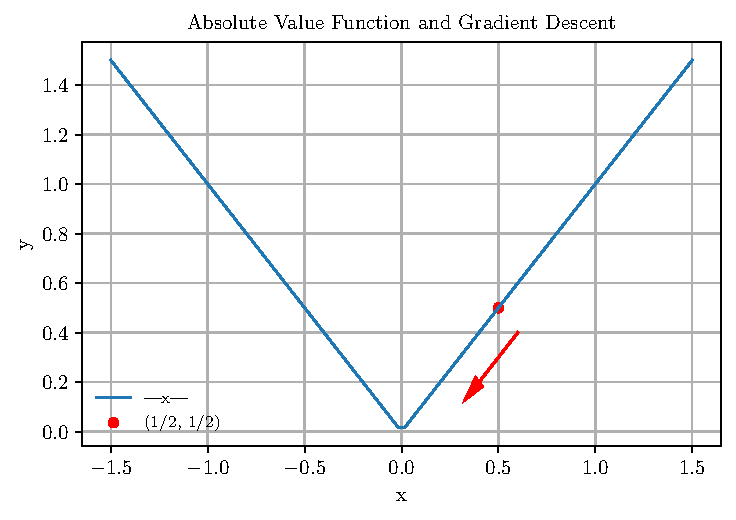
\includegraphics[width=0.7\textwidth]{plots/abs_val_func.pdf}
    \caption{The absolute value function $|x|$ and Gradient Descent with
        $x_0 = \frac{1}{2}$ and $t_k = 1$.
        We see that the Gradient jumps from $-1$ to $1$ at $x = 0$.
    }
    \label{fig:abs_value_function}
\end{figure}

In the example of the absolute value function $f(x) = |x|$,
Gradient Descent will oscillate forever,
with \emph{any constant step size} $t_k$.
The reason for the failure is that the gradient $\nabla f$
does not smoothly change at $x = 0$ but jumps from $-1$ to $1$
no matter how close the algorithm gets to the minimum $x = 0$.
This violates the condition that $\nabla f = 0$ at the minimum,
since $f$ is not differentiable
at $x = 0$.
One possible solution is to \emph{decay} the step size
$t_k$ during the optimization process.
However, the nature of this decay must be carefully chosen
as it can lead to the method getting stuck before
reaching the minimum.

\subsection{Line Search}

A perhaps more elegant solution to the step size problem
is to simply \emph{search} for the best step size $t_k$
at every iteration.
In the example of Figure~\ref{fig:abs_value_function},
we would quickly find the global minimum at $x = 0$.

% Define exact line search, many function calls

% Armijo-Wolfe conditions (with images)

% Define inexact line search as "algorithm" block
% Explain why it works on non-smooth functions

% We now expand on the line search approaches for non-smooth optimization

% Explain that exact line search tries to find the global minimizer of f in the
% given search direction, potentially requiring many function evaluations
With an \emph{exact line search}, we attempt to solve the one-dimensional
subproblem
\begin{equation}
    t_k = \underset{t > 0}{\arg\min} \; f\bigl(x_k + t\, p_k\bigr),
\end{equation}
and use the resulting $t_k$ to update $x_{k+1} = x_k + t_k\, p_k$.
In Gradient Descent, an exact line search results in the
next gradient being orthogonal to the current gradient.
Often, this method quickly approaches a neighbourhood of the minimum
taking very large steps initially, but can end up
taking many small
`zig-zag' steps once near the minimum.
As search directions likely change in the next step anyways,
searching for the exact best step size may be unnecessary.
This motivates the use of an \emph{inexact line search},
which just searches for some `good enough' step size.

The greater problem faces by exact line search is that
non-smooth functions may have many local minima
along the search direction.
Jumping to this non-differentiable point is problematic
since we (theoretically) cannot compute the gradient at
the next point $x_{k+1}$.

\subsection{Armijo-Wolfe Conditions}
To quantify what a `good enough' step size is, we may use
the following two conditions:
\begin{align}
    f\bigl(x_k + t_k\,p_k\bigr)              & \le f(x_k)
    + c_1\, t_k \,\nabla f(x_k)^T p_k, \tag{Armijo}                                       \\[6pt]
    \nabla f\bigl(x_k + t_k\,p_k\bigr)^T p_k & \ge c_2 \,\nabla f(x_k)^T p_k. \tag{Wolfe}
\end{align}

Here $0 < c_1 < c_2 < 1$ are the Armijo and Wolfe parameters,
and $t_k$ is the step size.
The Armijo condition ensures that the step size $t_k$ results in
a sufficient decrease in the objective function $f$.
It is often convenient to evaluate as it only requires function
evaluations and the current (already computed) gradient $\nabla f(x_k)$.
However, the Armijo condition allows for arbitrarily small step sizes
which may result in the algorithm taking many very small steps
and thus converging slowly.
Figure~\ref{fig:armijo_condition} illustrates the Armijo condition
together with intervals of step sizes that satisfy it.

\begin{figure}
    \centering
    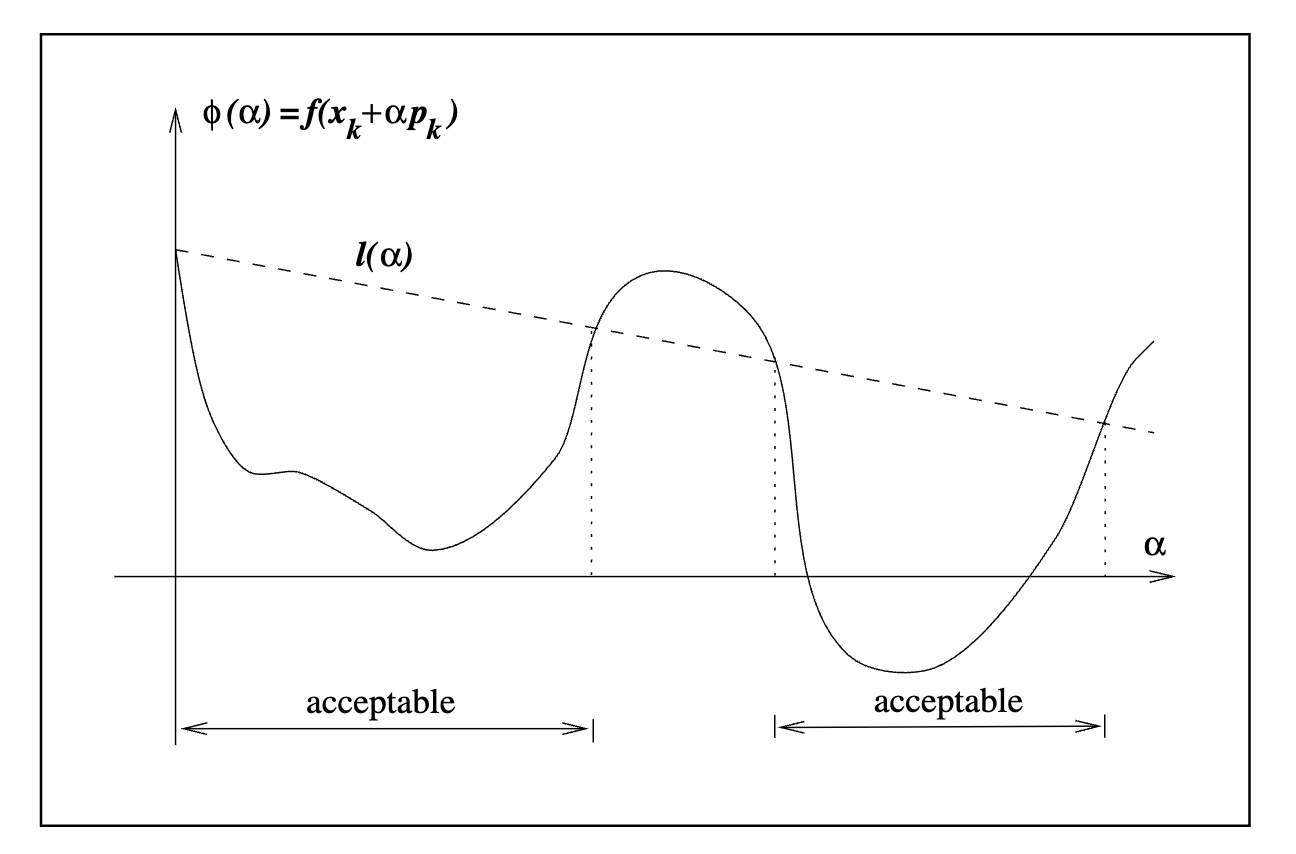
\includegraphics[width=0.7\textwidth]{plots/armijo_condition.png}
    \caption{Armijo condition ensuring sufficient decrease;
        Source: Numerical Optimization by Nocedal and Wright,
        Figure 3.3
    }
    \label{fig:armijo_condition}
\end{figure}

The Wolfe condition, sometimes known as the curvature condition
ensures that line search does not take too small steps.
Specifically, the left hand side
\begin{align*}
    \nabla f\bigl(x_k + t_k\,p_k\bigr)^T p_k
    = h'(t_k),
\end{align*}
is the derivative of the line search objective
$h(t) = f(x_k + t\,p_k)$
with respect to the step size $t_k$.
We can thus interpret this condition as ensuring that if
line search would still decrease the objective function
at $t_k$, then we should not stop yet.
It counters the problem faced by the Armijo condition,
but requires the computation of the gradient
$\nabla f\bigl(x_k + t_k\,p_k\bigr)$
at every new
point in the line search objective and is thus
costly to evaluate.
Other inexact line search algorithms often only rely on the
Armijo condition for this reason.
Figure~\ref{fig:wolfe_condition} illustrates the Wolfe condition.

\begin{figure}
    \centering
    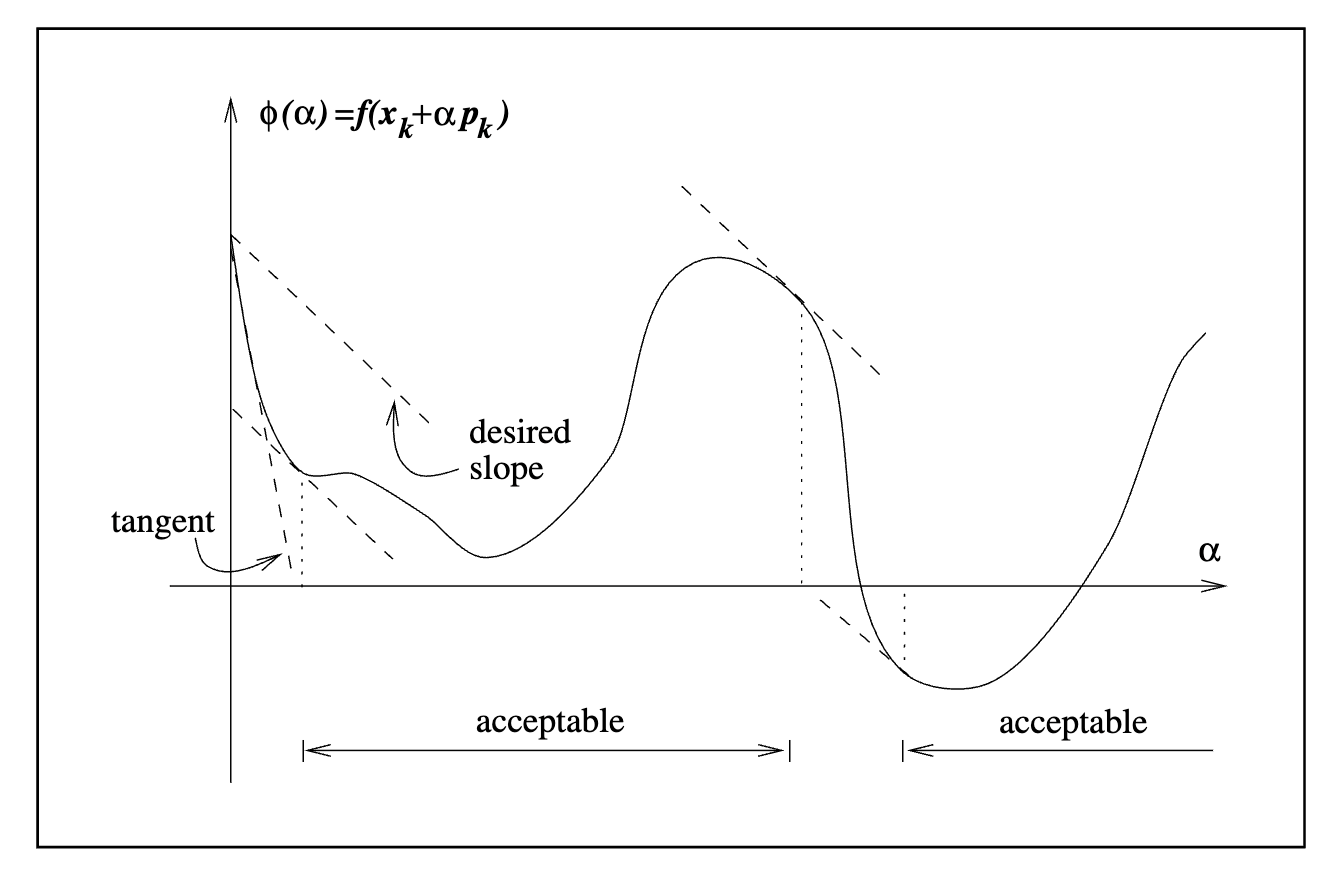
\includegraphics[width=0.8\textwidth]{plots/wolfe_condition.png}
    \caption{The Wolfe/Curvature condition;
        Source: Numerical Optimization by Nocedal and Wright,
        Figure 3.4}
    \label{fig:wolfe_condition}
\end{figure}

\subsection{Inexact Line Search Algorithm}

Using these two conditions, we can construct an inexact line search algorithm
known as the \emph{Armijo-Wolfe line search} as follows.
An important result is that the inexact ``Armijo-Wolfe'' line search
when used with the BFGS algorithm, shows better scaling of the
convergence rate when increasing the dimensionality $n$ in the
non-smooth problem of minimizing the euclidean norm
\begin{align*}
    \min_{x \in \mathbb{R}^n}
    \sqrt{x_1^2 + x_2^2 + \ldots + x_n^2}.
\end{align*}

\begin{algorithm}[htbp]
    \caption{Inexact ``Armijo-Wolfe'' line search}
    \SetAlgoLined
    Choose $0 < c_1 < c_2 < 1$, $t = 1$ \\
    $\alpha \gets 0$, $\beta \gets +\infty$ \\
    \Repeat{}{
        \textbf{if} $A(t)$ fails, \\
        \qquad $\beta \gets t$ \\
        \textbf{else if} $W(t)$ fails, \\
        \qquad $\alpha \gets t$ \\
        \textbf{else}, \\
        \qquad stop \\
        \textbf{if} $\beta < +\infty$, \\
        \qquad $t \gets (\alpha + \beta)/2$ \\
        \textbf{else}, \\
        \qquad $t \gets 2\alpha$
    }
    \label{alg:inexact_line_search}
\end{algorithm}

\end{document}